\documentclass[11pt,a4paper]{article}
\usepackage[utf8]{inputenc}
\usepackage[T1]{fontenc}
\usepackage{amsmath}
\usepackage{amsfonts}
\usepackage{amssymb}
\usepackage[left=3.0cm, right=3.0cm, top=3.0cm, bottom=3.0cm]{geometry}
\usepackage{xcolor}
\usepackage{graphicx}
\usepackage{caption}
\usepackage{subcaption}
\usepackage{braket}

% include code listings
\usepackage{listings}

% Defining colors for syntax highlighting
\definecolor{codegreen}{rgb}{0,0.6,0}
\definecolor{codegray}{rgb}{0.5,0.5,0.5}
\definecolor{codepurple}{rgb}{0.58,0,0.82}
\definecolor{backcolour}{rgb}{0.95,0.95,0.92}

\lstdefinestyle{mystyle}{
	backgroundcolor=\color{backcolour},   
	commentstyle=\color{codegreen},
	keywordstyle=\color{magenta},
	numberstyle=\tiny\color{codegray},
	stringstyle=\color{codepurple},
	basicstyle=\ttfamily\footnotesize,
	breakatwhitespace=false,         
	breaklines=true,                 
	captionpos=b,                    
	keepspaces=true,                 
	numbers=left,                    
	numbersep=5pt,                  
	showspaces=false,                
	showstringspaces=false,
	showtabs=false,                  
	tabsize=2
}

\lstset{style=mystyle}
\captionsetup[lstlisting]{font={scriptsize}}

% header and footer
\usepackage{fancyhdr}
\pagestyle{fancy}
\fancyhf{}
\lhead{Michele Guadagnini}
\rhead{\today}
\lfoot{Ex 9 - Quantum Information and Computing 2020/2021}
\rfoot{Page \thepage}

\author{Michele Guadagnini - ID 1230663}
\title{\textbf{Exercise 9 \\ One-Dimensional Ising Model}}
\date{\today}

%File names must include your name, exercise number and codewords REPORT, and CODE.
%Example: Ex2-Rossi-REPORT.pdf
%The maximum length of the report is five pages
\begin{document}
\maketitle

\vspace{20pt}
\begin{abstract}
	The aim of this exercise is to solve a 1D Ising model with $N$ spin-1/2 particles, transverse field and nearest neighbor interaction. The solution is done by computing and diagonalizing the Hamiltonian matrix.
\end{abstract}

\section{Theory} %Explain briefly the theory you have based your solution on.

We consider a system made of $N$ spin-1/2 particles in a 1D lattice in presence of a transverse field, with nearest neighbor interaction and open boundary condition. The Hamiltonian of this system is the following:
\begin{equation}
H = \lambda \sum_{i=1}^{N} \sigma_{z}^{i} + \sum_{j=1}^{N-1} \sigma_{x}^{j} \sigma_{x}^{j+1} 
\label{eq:ham}
\end{equation}
where $\lambda$ is a parameter that describes the field strength with respect to interaction strength. 
$\sigma_{z}^{i}$ and $\sigma_{x}^{j}\sigma_{x}^{j+1}$ are the matrices of size $2^N$ that results from the direct (Kronecker) products of the corresponding Pauli matrices with some padding identity matrices, as reported in Equation \ref{eq:kron}.
\begin{equation} \label{eq:kron}
\begin{aligned}
\sigma_{z}^{i} &= ( \bigotimes_{j=1}^{i-1} \mathbb{I}_2 ) \otimes  \sigma_{z} \otimes ( \bigotimes_{j=i+1}^{N} \mathbb{I}_2 ) \\
\sigma_{x}^{j}\sigma_{x}^{j+1} &= ( \bigotimes_{i=1}^{j-1} \mathbb{I}_2 ) \otimes  \sigma_{x} \otimes \sigma_{x} \otimes ( \bigotimes_{i=j+2}^{N-1} \mathbb{I}_2 )
\end{aligned}
\end{equation}
Since in front of the interaction term we have $+$ sign, this is an \textit{anti-ferromagnetic} system.

A local basis of the Hilbert space of a single spin particle can be described as $B_i$ = \{$\ket{0}, \ket{1}$\}. From this basis we can express the one of the global system as a composition of multiple local bases by mean of Kronecker product. This will be useful when implementing the Hamiltonian matrix computation.

\section{Code Development} %Introduce strategies, tests, and report debugging problems, compilations options

\subsection{Design and Implementation}

In the implementation of this exercise some subroutines and functions coming from previous exercises have been reused: 
\begin{itemize}
	\item the subroutine that reads the configuration file with the parameters values, \textit{InitParamsFromFile}. The used parameters are: $N$, number of spin particles; $k$, number of eigenvalues to save; $\lambda$, field strength.
	\item the subroutines that diagonalize a real (\textit{DOUBLE PRECISION}) symmetric matrix, \textit{SymmetricEigenpairs}.
\end{itemize}

The main effort in solving this problem has been to find a way to efficiently compute the Hamiltonian matrix. This computation has been split in two independent functions, one for the field term, one for the interaction one.

\subsubsection{Field term}
Due to the Pauli matrix $\sigma_{z}$, we know that the field term is diagonal and that the \textit{j-esim} term of the matrix $\sigma_{z}^{i}$:
\begin{itemize}
	\item is $1$ if we apply $\ket{0}$ on the \textit{j-esim} local space;
	\item is $-1$ if we apply $\ket{1}$.
\end{itemize}
This produces a mathematical trick to compute the field term, consisting in initialize all the diagonal elements to $N$ and subtract $-2$ to the \textit{j-esim} element whenever a $\bra{1_j} \sigma_{z} \ket{1_j}$ appears. The implementation is reported in Listing \ref{lst:zsum}.
\lstinputlisting[language=FORTRAN, firstnumber=65, linerange={65-83}, caption=Computation of the Hamiltonian field term., label=lst:zsum]{Ex9-Guadagnini-SpinsHamiltonian-CODE.f90}

\subsubsection{Interaction term}
Regarding the interaction term, we notice that $\sigma_{x}^{i}$ is always zero apart from the matrix elements where $\bra{bra}$ and $\ket{ket}$ are different for the \textit{i-esim} particle. 
From this fact, as before, we can build a method based on the binary representation of the index of the global basis and the \textit{XOR} operation. The code is reported in Listing \ref{lst:xsum}.
\lstinputlisting[language=FORTRAN, firstnumber=85, linerange={85-103}, caption=Computation of the Hamiltonian interaction term., label=lst:xsum]{Ex9-Guadagnini-SpinsHamiltonian-CODE.f90}

\subsubsection{Scripting}
In order to automatize the running of the program with different $N$ and $\lambda$ values, a Python script, called \textit{Ex9-Guadagnini-Script-CODE.py}, has been created, that loops over the values of the two variables. 
It also saves the execution time of the program. Since the computation time does not depend on the value of $\lambda$, it computes the average time for a particular $N$.

Also the plotting has been automatized by creating a gnuplot script contained in the file \textit{Ex9-Guadagnini-LevelsPlot.gnuplot}.

\subsection{Debug and Test}

The program has been compiled and executed with the following commands:
\begin{lstlisting}[language=BASH,numbers=none]
	gfortran *CODE.f90 -o Ising1D.x -lblas -llapack -g -fcheck=all -Wall
	./Ising1D.x
\end{lstlisting}
Once checked that it was working correctly, it has been tested the maximum number of spin particles that is possible to simulate and the computation time by running the Python script. 
The plot of the timings is reported in Figure \ref{fig:timings}. The maximum $N$ used is $12$. We can, in principle, store in memory an Hamiltonian of size also $2^{14}$, since, with double precision numbers, it requires $2GB$ of RAM. 
However, looking at Figure \ref{fig:timings}, we can see that the computation time grows very fast with $N$, and by exploiting the fitted parameters we can estimate that, in this machine, even with $N=13$ it would take almost $30 min$ to complete a single step in the $\lambda$ grid space.

\begin{figure}
	\centering
	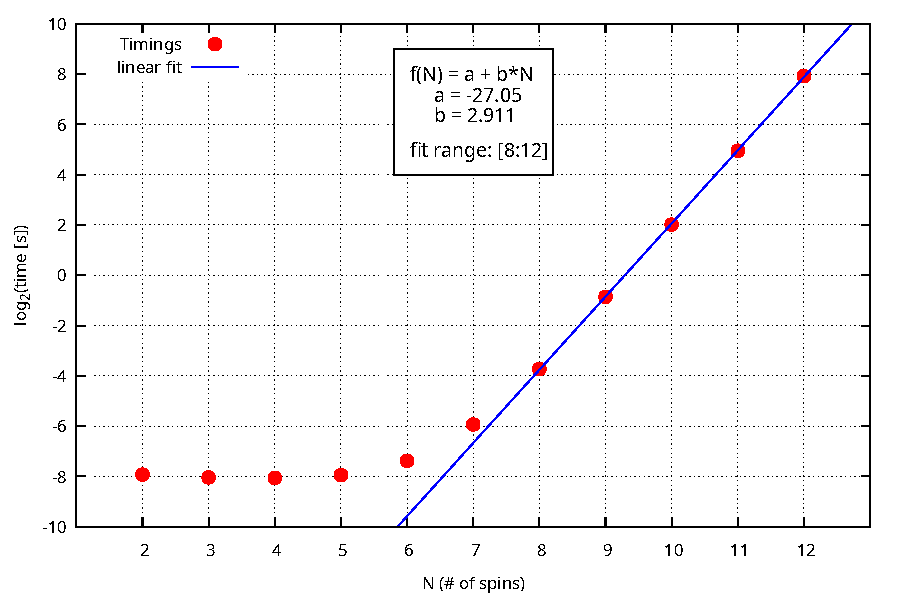
\includegraphics[width=0.75\linewidth]{Timings.pdf}
	\caption{$Log_2$ of the average computation times for different value of $N$. Timings are averaged over the $\lambda$ steps.}
	\label{fig:timings}
\end{figure}

\section{Results} %Present data and explain your results.

The computed eigenvalues have been plotted using the gnuplot script. Eigenvalues are also normalized by a factor of $\frac{1}{N-1}$ to better compare them. Two types of plots have been created: 
\begin{itemize}
	\item the first type reports up to the first $8$ eigenvalues in function of $\lambda$ for a particular system size $N$. A sample of all the plots of this kind created is reported in Figure \ref{fig:plotsN}. 
	\item the second type reports instead the same eigenvalue (i.e. ground state, first excited, ...) in function of $\lambda$ for all the tested $N$ values. A sample of this plots is reported in Figure \ref{fig:plotsk}.
\end{itemize}
A thing that arises looking at the pictures, in particular at Figure \ref{fig:N3}, is that for $\lambda$ = 0, so without an external field, the eigenvalues show degeneracy, while with $\lambda$ increasing they start to separate more and more. 

% figure and subfigures
\begin{figure}
	\centering
	\begin{subfigure}{0.49\textwidth}
		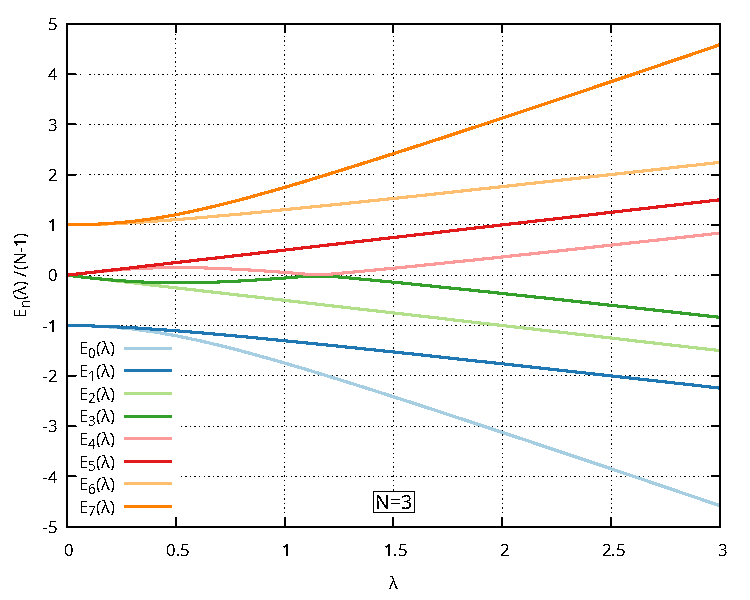
\includegraphics[width=1\linewidth]{Plots/EigVals_N03.pdf}
		\caption{N=3}
		\label{fig:N3}
	\end{subfigure}%
	\hfill
	\begin{subfigure}{0.49\textwidth}
		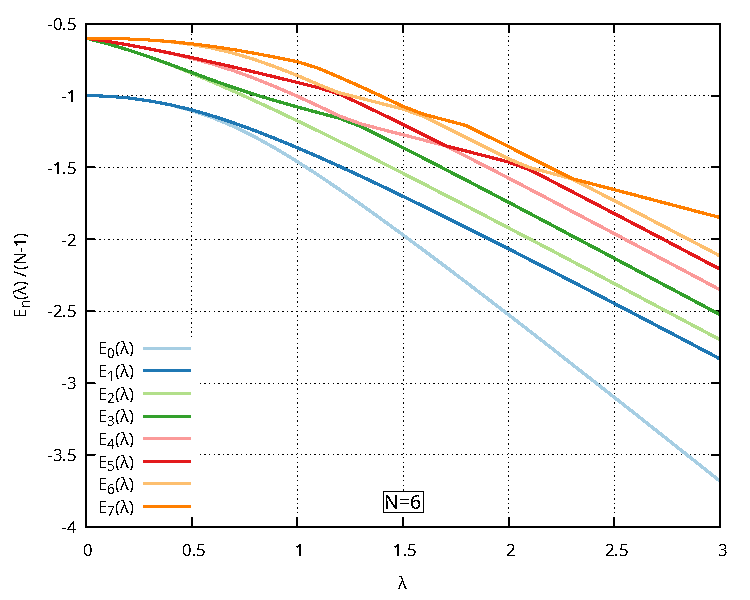
\includegraphics[width=1\linewidth]{Plots/EigVals_N06.pdf}
		\caption{N=6}
		\label{fig:N6}
	\end{subfigure}
	\begin{subfigure}{0.49\textwidth}
		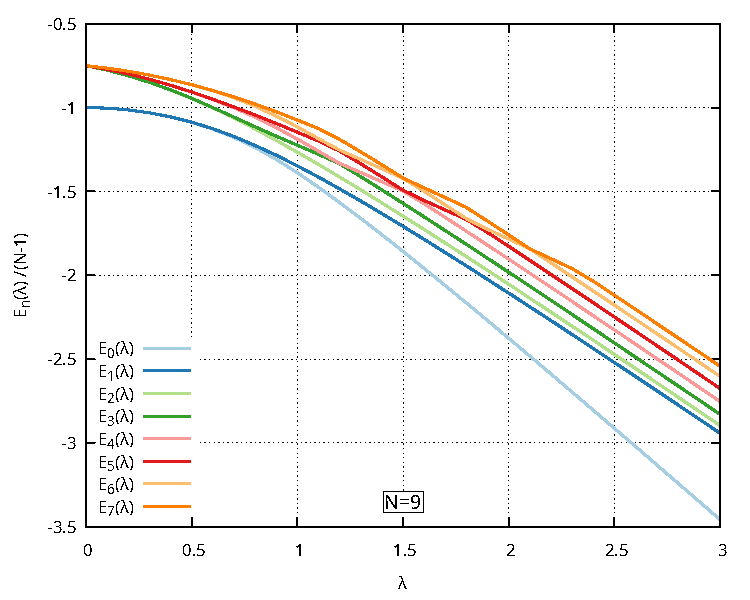
\includegraphics[width=1\linewidth]{Plots/EigVals_N09.pdf}
		\caption{N=9}
		\label{fig:N9}
	\end{subfigure}
	\hfill
	\begin{subfigure}{0.49\textwidth}
		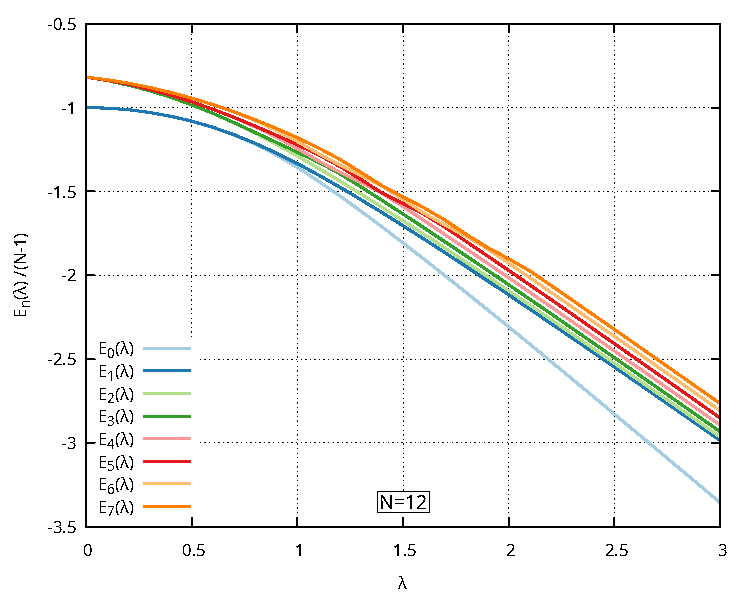
\includegraphics[width=1\linewidth]{Plots/EigVals_N12.pdf}
		\caption{N=12}
		\label{fig:N12}
	\end{subfigure}
	\caption{Grid of plots of the first $8$ eigenvalues corresponding to the first $8$ excited states for several values of $N$.}
	\label{fig:plotsN}
\end{figure}

% figure and subfigures
\begin{figure}
	\centering
	\begin{subfigure}{0.49\textwidth}
		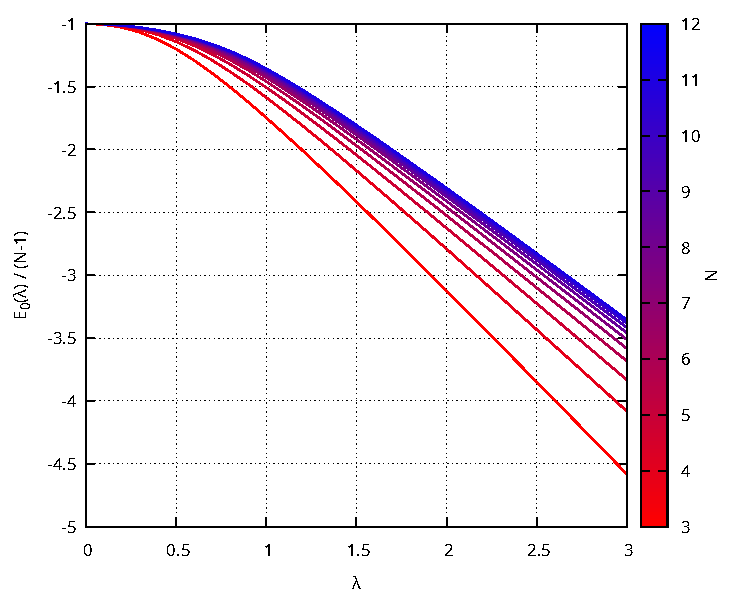
\includegraphics[width=1\linewidth]{Plots/EigVals_k00.pdf}
		\caption{$E_0$, ground state.}
		\label{fig:k0}
	\end{subfigure}%
	\hfill
	\begin{subfigure}{0.49\textwidth}
		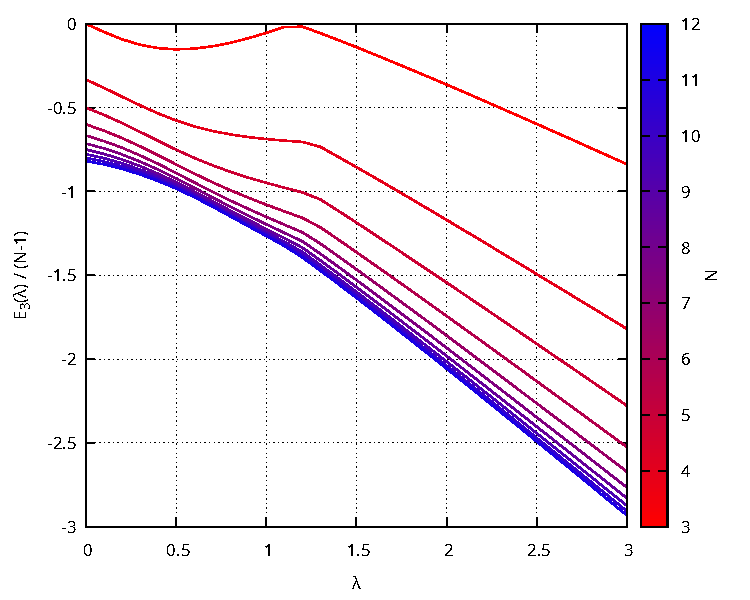
\includegraphics[width=1\linewidth]{Plots/EigVals_k03.pdf}
		\caption{$E_3$, third excited.}
		\label{fig:k3}
	\end{subfigure}
	\caption{Grid of plots of the ground state and the third excited eigenvalues in function of $\lambda$ for all the values of $N$ from $3$ to $12$.}
	\label{fig:plotsk}
\end{figure}

\section{Self-evaluation} %What have you learned? What can be done next? What went wrong and why?

In this exercise we exploited the binary representation of the indexes to compute the Hamiltonian in a more efficient way with respect to do all the tensor products to pad the Pauli matrices. It would be interesting to evaluate the gap in terms of computational time between these two procedures.
To improve the execution time estimation we could have saved also the variance of the computed means in order to improve the fit and the plot with empirical errors.

	
\end{document}
